\documentclass[conference]{IEEEtran}
\usepackage{ifpdf}
\usepackage{booktabs}
\usepackage{cite}
\usepackage[cmex10]{amsmath}
\usepackage{amsfonts}
\usepackage{url}
\usepackage{color}
\usepackage[utf8]{inputenc}
\usepackage{algpseudocode}
\usepackage{algorithm}
\usepackage{booktabs}
\usepackage{tabularx}
\usepackage{multicol}
\usepackage{bm}
\usepackage{multirow}
\usepackage{array}
\usepackage{epstopdf}
\usepackage{siunitx}
\ifCLASSINFOpdf
   \usepackage[pdftex]{graphicx}
  % declare the path(s) where your graphic files are
   \graphicspath{{figures/png/}}
  % and their extensions so you won't have to specify these with
  % every instance of \includegraphics
  \DeclareGraphicsExtensions{.png}
\else
  % or other class option (dvipsone, dvipdf, if not using dvips). graphicx
  % will default to the driver specified in the system graphics.cfg if no
  % driver is specified.
  \usepackage[dvips]{graphicx}
  % declare the path(s) where your graphic files are
  \graphicspath{{figures/eps/}}
  % and their extensions so you won't have to specify these with
  % every instance of \includegraphics
  \DeclareGraphicsExtensions{.eps}
\fi
\usepackage{epsfig}
\newcolumntype{M}{>{$\vcenter\bgroup\hbox\bgroup}c<{\egroup\egroup$}}
\newcommand{\etal}{\textit{et al.}}

\DeclareMathOperator*{\argmin}{argmin}
\newcommand\undermat[2]{%
	\makebox[0pt][l]{$\smash{\underbrace{\phantom{%
					\begin{matrix}#2 \end{matrix}}}_{\text{$#1$}}}$}#2}
\usepackage[font=small, labelfont=bf, format=plain, labelsep=space, figurename=Figure, tablename=Table]{caption}\usepackage[labelfont=rm, labelformat=parens, labelsep=space]{subcaption}

\begin{document}
%
% paper title
% Titles are generally capitalized except for words such as a, an, and, as,
% at, but, by, for, in, nor, of, on, or, the, to and up, which are usually
% not capitalized unless they are the first or last word of the title.
% Linebreaks \\ can be used within to get better formatting as desired.
% Do not put math or special symbols in the title.
\title{Morphological component analysis for sparse regularization in plane wave imaging}

\author{\IEEEauthorblockN{Adrien Besson\IEEEauthorrefmark{1},
Rafael E. Carrillo\IEEEauthorrefmark{1}, 
Dimitris Perdios\IEEEauthorrefmark{1},
Eric F. Bezzam\IEEEauthorrefmark{2},
Marcel Arditi\IEEEauthorrefmark{1},
Yves Wiaux\IEEEauthorrefmark{3},} and 
Jean-Philippe Thiran\IEEEauthorrefmark{1}\IEEEauthorrefmark{4}
\IEEEauthorblockA{\IEEEauthorrefmark{1}Signal Processing Laboratory (LTS5),
Ecole Polytechnique F\'{e}d\'{e}rale de Lausanne,
Lausanne, Switzerland\\}
\IEEEauthorblockA{\IEEEauthorrefmark{2}Audiovisual Communications Laboratory (LCAV),
Ecole Polytechnique F\'{e}d\'{e}rale de Lausanne,
Lausanne, Switzerland\\}
\IEEEauthorblockA{\IEEEauthorrefmark{3}Institute of Sensors, Signals and Systems, Heriot-Watt University, Edinburgh, UK\\}
\IEEEauthorblockA{\IEEEauthorrefmark{4}Department of Radiology, University Hospital Center (CHUV) and University of Lausanne (UNIL), Lausanne, Switzerland}}
\maketitle

\begin{abstract}
Classical ultrasound image reconstruction mainly relies on the well-known Delay-And-Sum (DAS) beamforming for its simplicity and real-time capability. Sparse regularization methods propose an alternative to DAS which lead to a better inversion of the ill-posed problem resulting from the acoustic wave propagation. In the following work, a new sparse regularization method is proposed which includes a component-based modelling of the radio-frequency images as well as a point-spread-function-adaptive sparsity prior. The proposed method, evaluated on the PICMUS dataset, outperforms the classical DAS in terms of contrast and resolution.   
\end{abstract}

\begin{IEEEkeywords}
Plane wave, Sparse regularization, Compressed sensing
\end{IEEEkeywords}

\IEEEpeerreviewmaketitle

\section{Introduction}
\par Classical ultrasound (US) imaging relies on the well-known Delay-And-Sum (DAS) beamforming which is based on compensating the hyperbolic travel-time curve induced by the propagation from any inhomogeneity in the imaged medium.
\par Such a model is used in many ultrasound modalities due to its ability to be computed in real time. Indeed, DAS beamforming is highly parallelisable and requires only few delay calculations per pixel. However, it has been demonstrated that DAS is a roughly approximated solution of the ill-posed inverse problem induced by the propagation~\cite{David_JASA_2015}. 
\par Sparse regularization methods appear as an alternative to DAS in which the solution of the inverse problem is retrieved by means of an optimization algorithm. The idea behind these approaches resides in assuming that the image under scrutiny is sparse under a given model. Following this model, the optimization problem searches for the sparsest solution under the data fidelity constraint.
\par In US imaging, sparse regularization have been extensively used with various models for the sparsity priors. Liebgott~\textit{et~al.}~\cite{Liebgott_Ult_2013} use the sparsity of backscattered echoes in the wave atom frame to reduce the number of required echoes in a pre-beamforming step. In a post-beamforming step, a sparsity prior of Radio-Frequency~(RF) images has been exploited in various models such as: Fourier basis~\cite{Quinsac2012}, wavelet basis~\cite{Quinsac2012}, sparsity averaging model~\cite{Carrillo_IUS_2015, Besson_ICIP_2016}, $\alpha-$stable distribution~\cite{Dobigeon2012} or more recently in learned dictionaries~\cite{Lorintiu_TMI_2015}.
\par In our previous works, it has been shown that sparse regularization outperforms classical approaches in terms of image quality~\cite{Carrillo_IUS_2015, Besson_EUSIPCO_2016, Besson_UFFC_2016}. Several drawbacks of sparse regularization have also been enlightened which may degrade the quality of the reconstruction. Firstly, the use of the same sparsity prior for the whole image is intrinsically incompatible with US imaging in which the point-spread-function (PSF) varies across the imaging range. Secondly, modelling the complexity of RF images with only one sparsifying model is a too simplistic approach.
\par In this paper, we propose a more elaborated sparse regularization approach based on dividing the desired image into two components, namely a bright reflector part and a background part. The two components are sparse under different models, in a simialr manner as described in the morphological component analysis framework (MCA)~\cite{Starck2004}. In addition, a PSF-adaptive prior is also proposed. Section~\ref{sec:sparse_regularization} reviews the sparse regularization method. The proposed approach is described in Section~\ref{sec:proposed_approach} and evaluated on the PICMUS dataset in Section~\ref{sec:results}. Concluding remarks are given in Section~\ref{sec:Conc}.
%%%%%%%%%%%%%%%%%%%%%%%%%%%%%%%%%%%%%%%%%%%%%%%%%%%%%%%%%%%%%%%%%%%%%%%%%%%%%%%%
\section{Sparse regularization for ultrasound imaging}
\label{sec:sparse_regularization}
\subsection{General framework}
\label{subsec:general_framework}
Sparse regularization methods aim at proposing an alternative to classical image reconstruction methods. Formally, let us denote as $\bm{r} \in \mathbb{R}^M$ the element raw data and as $\bm{s} \in \mathbb{R}^N$ the desired RF image.
The idea behind sparse regularization is to exploit sparsity of the RF image in a given model in order to invert an ill-posed problem. Thus, it relies on two pillars:
\begin{itemize}
	\item The ability to express an operator $\mathsf{H} \in \mathbb{R}^{M \times N}$ such that $\bm{r} = \mathsf{H} \bm{s} + \bm{n}$. $\mathsf{H}$ is denoted as the measurement operator.
	\item The ability to find $\mathsf{\Psi} \in \mathbb{R}^{N \times L}$ such that $\mathsf{\Psi}^\dagger \bm{s}$ is sparse, where $\mathsf{\Psi}^\dagger$ denotes the adjoint of $\mathsf{\Psi}$.
\end{itemize}
The desired image is then reconstructed by solving the following analysis-based convex problem:
\begin{equation}\label{cs6}
\min_{\bar{\bm{s}}\in\mathbb{C}^{N}}\|\mathsf{\Psi}^{\dagger}\bar{\bm{s}}\|_{1}
\textnormal{ subject to }\| \bm{r}-\mathsf{H}\bar{\bm{s}}\|_{2}\leq\epsilon,
\end{equation}
\subsection{Measurement operator in PW imaging}
\label{subsec:measop_PWimaging} 
The measurement operator for PW imaging has been derived in previous works~\cite{Besson_ICIP_2016, Besson_EUSIPCO_2016}. Formally, let us denote by $r \left(x_i, t\right)$ the element raw data received at time $t$ by a transducer positioned at $x_i$. Let us also define $s \left(x, z\right)$ the RF-image corresponding to the point in the medium located at $\left(x, z\right)$ and consider a steered plane wave (PW) insonification with angle $\theta$. It can be demonstrated that the following equation holds:
\begin{equation}
\label{eq_inv_problem_cont_domain}
r \left( x_i, t \right) = \iint \limits_{ \left( x, z \right) \in \Omega \left( x_i, t \right)} s \left( x, z \right) dx dz, 
\end{equation} 
where $\Omega \left(x_i, t \right) = \left\lbrace \left( x, z\right) \; | \; t = t_{Rx} \left( x_i, x, z \right) + t_{Tx} \left( x, z \right) \right\rbrace$, in which $t_{Rx} \left( x_i, x, z \right)~=~\sqrt{\left( x - x_i\right)^2 + \left( z - z_i \right)^2} / c$ and $t_{Tx}\left(x, z \right)~=~z \cos \theta / c + x \sin \theta / c$ denote the delays on receive and transmit respectively.
The discretization of Equation~\eqref{eq_inv_problem_cont_domain} on the two grids defined by the element raw data and the desired image leads to the following inverse problem:
\begin{equation}
\bm{r} = \mathsf{H} \bm{s} + \bm{n}.
\end{equation}
\subsection{Sparsity prior}
\label{subsec:sparsity_prior}
\par In the literature, various sparsifying models have already been proposed mainly relying on wavelet-based models~\cite{Schiffner_IUS_2012, David_JASA_2015, Chen2015}. In our previous work, we suggested to use a concatenation of wavelet bases since it exhibits better reconstruction results than traditional wavelet-based models. The model, denoted as Sparsity Averaging (SA) model is composed of the concatenation of Daubechies wavelet transforms with different wavelet mother functions ranging from Daubechies 1~(Db1) to Daubechies 8 ~(Db8)~\cite{Carrillo_SPL_2012, Carrillo_IUS_2015, Besson_ICIP_2016, Besson_EUSIPCO_2016}. Thus,
\begin{equation}\label{sara}
\mathsf{\Psi} = \frac{1}{\sqrt{q}} [\mathsf{\Psi_{1}},...,\mathsf{\Psi_{q}}],
\end{equation}
where $q=8$ and $\mathsf{\Psi_i}$ denotes $i$-th Daubechies wavelet. 
\subsection{Limits of sparse regularization}
\label{subsec:limits_sparse_reg}
It has been demonstrated that sparse regularization approach outperforms classical approaches in terms of image quality. However, the methods described above suffer from two main limitations which are intrinsic to US images. Firstly, ultrasound images are characterized by spatially varying statistics. This aspect is visible in the shape of the Point-Spread-Function~(PSF) which varies in both the lateral and the axial dimensions. Such a variation is not in line with the sparsity prior that assumes the same statistics in the whole image. This leads to problems in the reconstruction of fully-developed speckle \cite{Besson_UFFC_2016}.
In addition, US images are composed of various components such as fully developed speckle, bright reflectors and structural parts \textit{e.g.} carotid arteries, each of these sparse in a different model. Assuming a sparsity prior in a single model is thus a too simplistic assumption which is refined in the proposed approach.
%%%%%%%%%%%%%%%%%%%%%%%%%%%%%%%%%%%%%%%%%%%%%%%%%%%%%%%%%%%%%%%%%%%%%%%%%%%%%%%%
\section{Proposed approach}
\label{sec:proposed_approach}
In this section, problem \eqref{cs6} is generalized to:
\begin{equation}
\label{eq_mca_inv_problem}
\min_{\bar{\bm{s}}\in\mathbb{C}^{N}} f(\bar{\bm{s}})
\textnormal{ subject to }\| \bm{r}-\mathsf{H}\bar{\bm{s}}\|_{2}\leq\epsilon,
\end{equation}
where the prior function $f(.)$ will be defined in the following.
\subsection{Morphological component analysis}
\label{subsec:MCA}
The first improvement resides in modelling the RF image as a sum of a background and a bright reflector components. Such an approach has raised more and more interest in US imaging~\cite{BZhang_IUS_2015, Yankelevsky_arxiv_2016, Szasz_Ult_2016}. Formally, the equation $\bm{s} = \bm{s_b} + \bm{s_r}$ where $\bm{s_b}$ and $\bm{s_r}$ denote the background and the bright reflector components respectively can be written.
Each component is sparse in a given model denoted as respectively $\mathsf{\Psi_b}$ and $\mathsf{\Psi_r}$. This leads to 
\begin{equation}
\label{eq:f}
f(\bm{s_b}, \bm{s_r}) = || \mathsf{\Psi_b} \bm{s_b} ||_1 + || \mathsf{\Psi_r} \bm{s_r} ||_1.
\end{equation}
Problem \eqref{eq_mca_inv_problem}, with $f()$ defined in Equation \eqref{eq:f}, is similar to the MCA problem~\cite{Starck2004}.
\subsection{Adaptive sparsity prior}
\label{subsec:local_sparsity_prior}
The prior function defined in Equation \eqref{eq:f} encapsulates a component-based model of the RF image. However, it does not take into account the spatial variability of the PSF which results in a statistical variability across the US image. In addition, it is supposed that the apodization compensates for the lateral variability of the PSF at a given depth~\cite{Michailovich_TMI_2005}. Taking into account the above assumptions, the RF image is divided into non-overlapping segments in the axial dimension where the PSF is considered as quasi-stationary~\cite{Michailovich_TMI_2005} and a sparsity prior is applied onto each segment independently.
\par Formally, if $\bm{s_b}$ and $\bm{s_r}$ are divided into $L$ non-overlapping segments, the prior function becomes 
\begin{equation}
\label{eq_f_mca_l1}
f \left(\bm{s_{b}}, \bm{s_r} \right) = \sum \limits_{i = 1}^{L} \left(|| \mathsf{\Psi_b} \bm{s_{b_i}} ||_1 + || \mathsf{\Psi_r} \bm{s_{r_i}} ||_1\right),
\end{equation}
where $\bm{s_{b_i}}$ and $\bm{s_{r_i}}$ for $i$ between $1$ and $L$ correspond to the different segments.
\par Instead of using the $\ell_1$-norm as a sparsity promoting norm, the $\ell_p$-norm, with $p < 1$, is considered in the proposed method. This choice is justified by the fact that it better approximates the $\ell_0$-norm. Moreover, a closed-form formulation for the shrinkage operator associated with the power p of the $\ell_p$-norm has been derived recently by Woodworth~\textit{et~ al.}~\cite{Woodworth_IP_2016}. Including this consideration in Equation \eqref{eq_f_mca_l1} leads to the following formulation of the prior function:
\begin{equation}
\label{eq_f_mca_tot}
f \left(\bm{s_{b}}, \bm{s_r} \right) = \sum \limits_{i = 1}^{L} \left(|| \mathsf{\Psi_b} \bm{s_{b_i}} ||_p^p + || \mathsf{\Psi_r} \bm{s_{r_i}} ||_p^p\right).
\end{equation}
\subsection{The proposed problem}
\label{subsec_proposed_pb}
Given the function defined in Equation \eqref{eq_f_mca_tot}, it is possible to derive the following problem:
\begin{equation}
\label{eq_mca_inv_problem_tot}
\min_{\bar{\bm{s_b}}, \bar{\bm{s_r}}} f(\bar{\bm{s_b}}, \bar{\bm{s_r}})
\textnormal{ subject to }\| \bm{r}-\mathsf{H}\left(\bar{\bm{s_b}} + \bar{\bm{s_r}}\right)\|_{2}\leq\epsilon.
\end{equation}
Problem \eqref{eq_mca_inv_problem_tot} is a classical analysis-based problem, solved using the Douglas-Rachford algorithm~\cite{Combettes_TSP_2007}.
\subsection{Adjustable image display}
\label{subsec_final_image_display}
The solution of Problem \eqref{eq_mca_inv_problem_tot} provides the two components $\bm{s_b}$ and $\bm{s_r}$. In order to control the amount of speckle in the desired image, an approach similar to the one proposed by Szasz~\textit{et~al.}~\cite{Szasz_Ult_2016} is used. A parameter $\gamma \in \left[0,1\right]$ is introduced such that: 
\begin{equation}
\bm{s_d} = \gamma \bm{s_r} + (1-\gamma) \bm{s_b}.
\end{equation}
If some speckle is desired in the displayed image, then $\gamma$ has to be set close to 0, otherwise it can be set close to 1.
%%%%%%%%%%%%%%%%%%%%%%%%%%%%%%%%%%%%%%%%%%%%%%%%%%%%%%%%%%%%%%%%%%%%%%%%%%%%%%%%
\section{Results}
\label{sec:results}
The proposed approach is evaluated on the PICMUS dataset in the following categories: 1 PW, 3 PWs and 11PWs. The angles for the 11 PWs experiment are chosen uniformly across the angle range. For the 3PWs experiment, the considered angles are chosen to be \SIlist{-0.43; 0; 0.43}{\degree}. In all the experiments, $\mathsf{\Psi_b}$ is the SA model described in Section \ref{subsec:sparsity_prior} and $\mathsf{\Psi_r}$ is the Dirac basis. As a reference, the classical DAS is also computed on the dataset for each experiment.
\newlength{\CarotidFigWidth} \setlength{\CarotidFigWidth}{0.3\textwidth}
\newlength{\CarotidFigHeight}
\settoheight{\CarotidFigHeight}{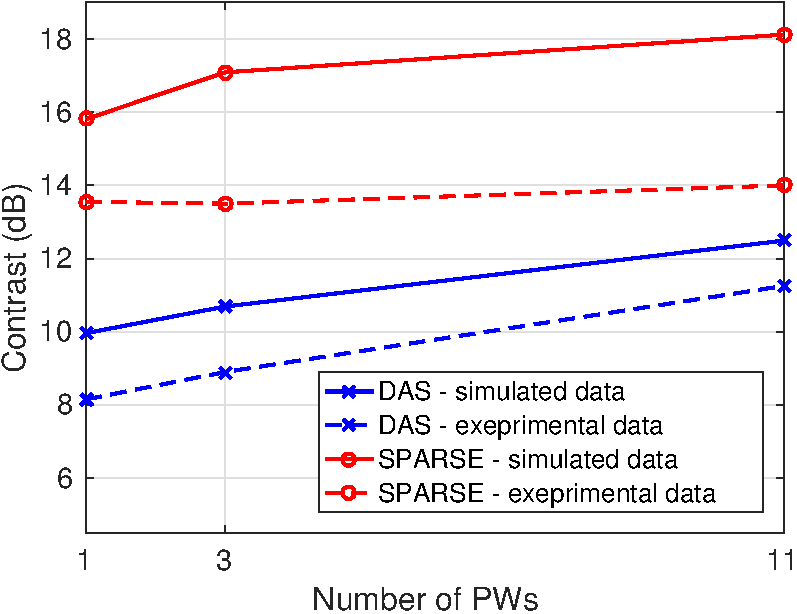
\includegraphics[width=\CarotidFigWidth]{figures/CR_PICMUS.pdf}} 
\begin{figure*}[htb]
	% Maximum length
	\hfill%
	\subcaptionbox{\label{fig:contrast} }{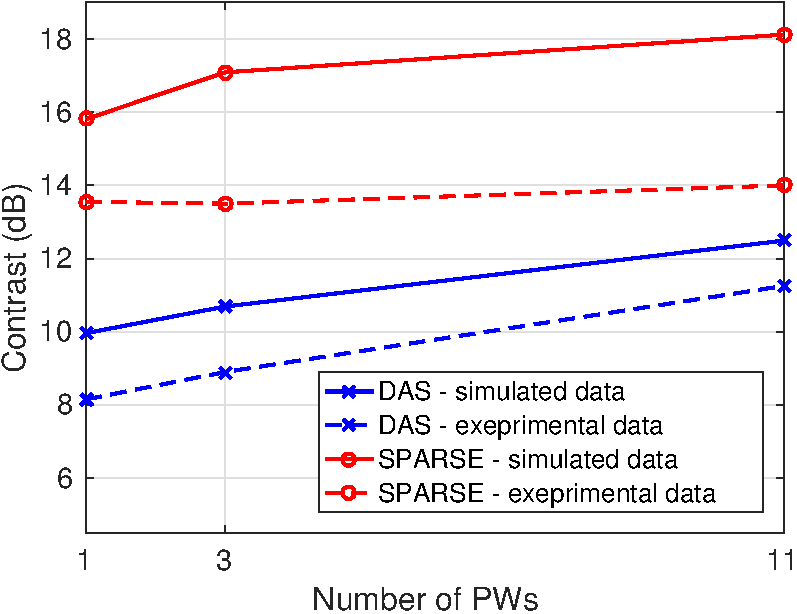
\includegraphics[height=\CarotidFigHeight]{figures/CR_PICMUS.pdf}}\hfill%
	\subcaptionbox{\label{fig:axial_res} }{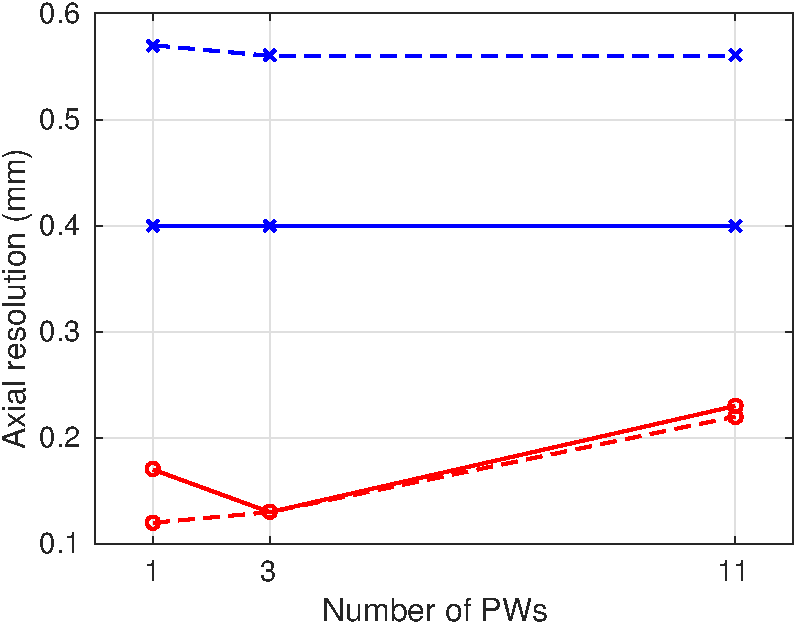
\includegraphics[height=\CarotidFigHeight]{figures/AxialRes_PICMUS.pdf}}\hfill%
	\subcaptionbox{\label{fig:lat_res}}{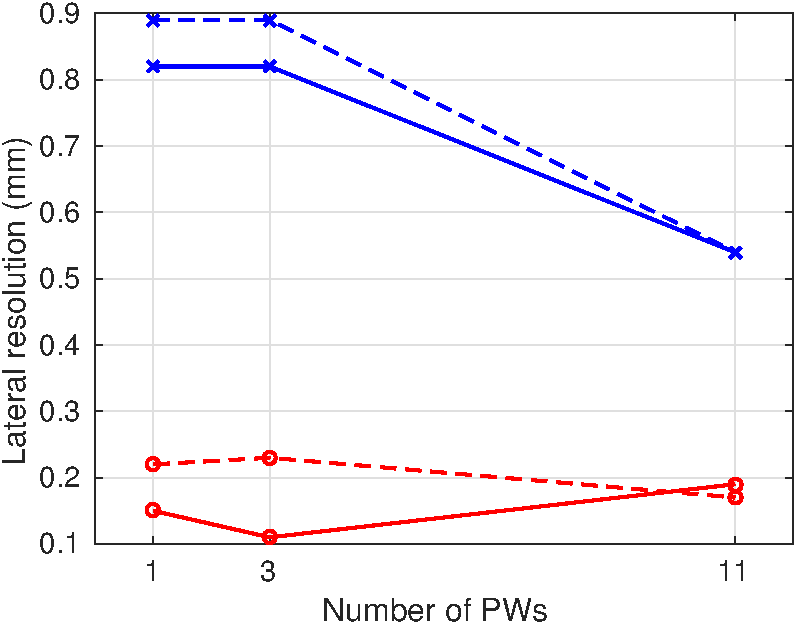
\includegraphics[height=\CarotidFigHeight]{figures/LateralRes_PICMUS.pdf}}\hfill%
	\caption{(a) Contrast, (b) axial resolution and (c) lateral resolution on simulated (solid line) and experimental (dashed line) PICMUS datasets for the classical DAS (blue cross) and the proposed method (red circle) for 1, 3 and 11 PWs.}
\end{figure*}
\newlength{\SimFigWidth} \setlength{\SimFigWidth}{0.22\textwidth}
\newlength{\SimFigHeight}
\settoheight{\SimFigHeight}{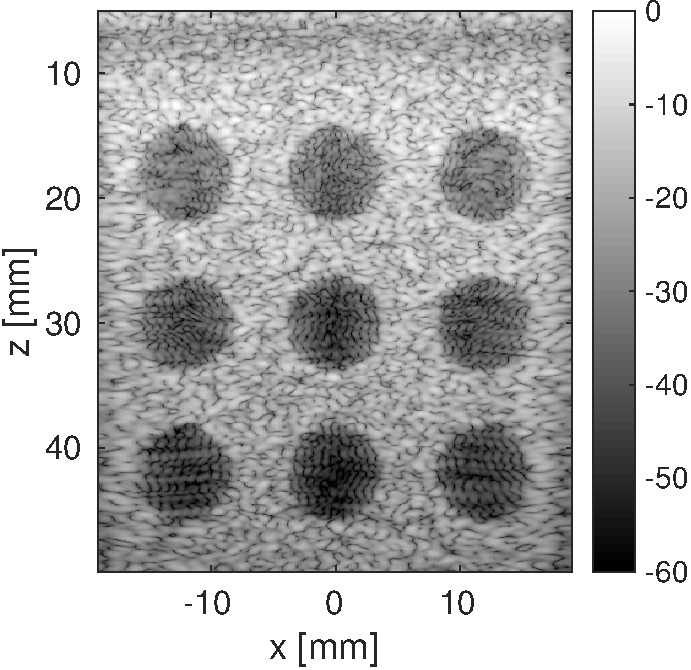
\includegraphics[width=\SimFigWidth]{figures/DAS_CR_1PW.pdf}} 
\begin{figure*}[htb]
	% Maximum length
	\hfill%
	\subcaptionbox{ }{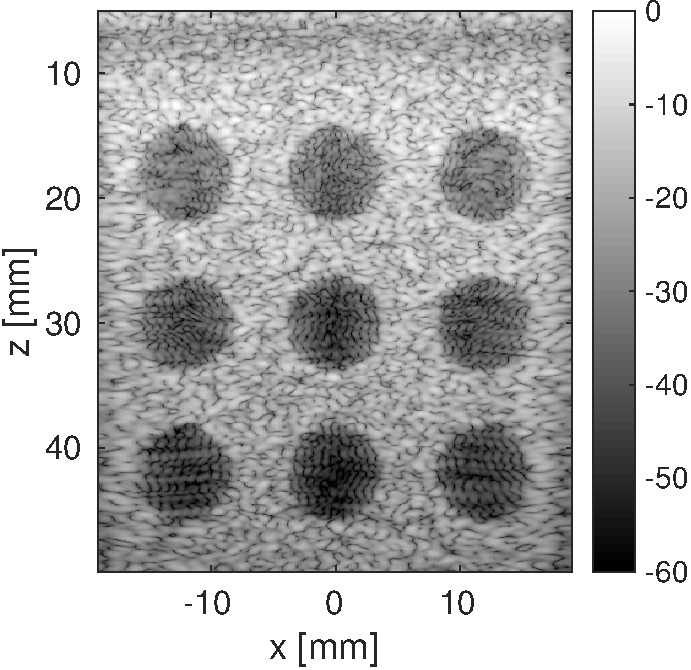
\includegraphics[height=\SimFigHeight]{figures/DAS_CR_1PW.pdf}}\hfill%
	\subcaptionbox{ }{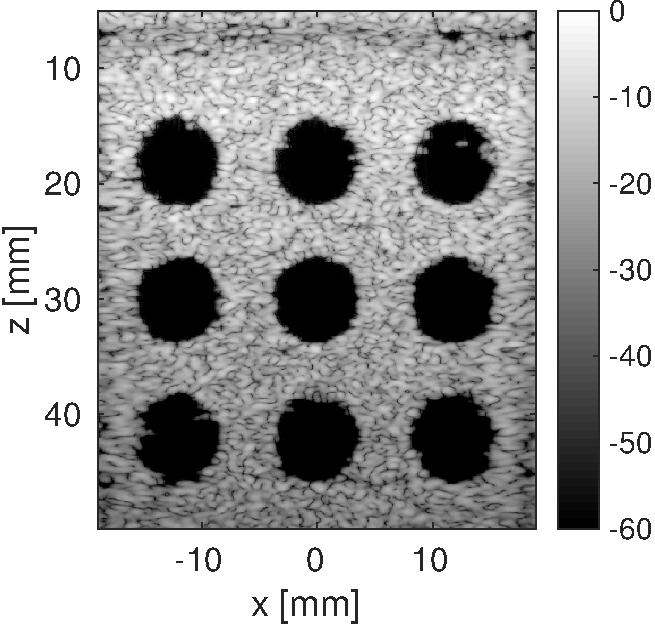
\includegraphics[height=\SimFigHeight]{figures/MCA_CR_1PW.pdf}}\hfill%
	\subcaptionbox{ }{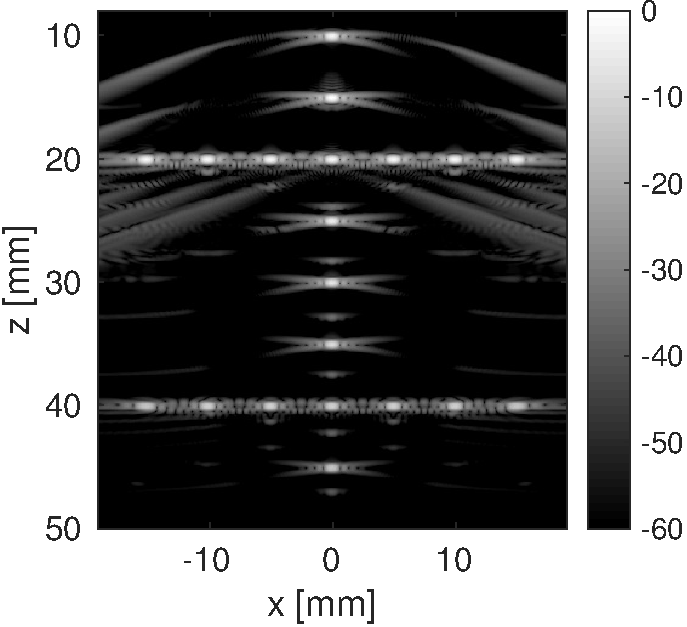
\includegraphics[height=\SimFigHeight]{figures/DAS_res_1PW.pdf}}\hfill%
	\subcaptionbox{}{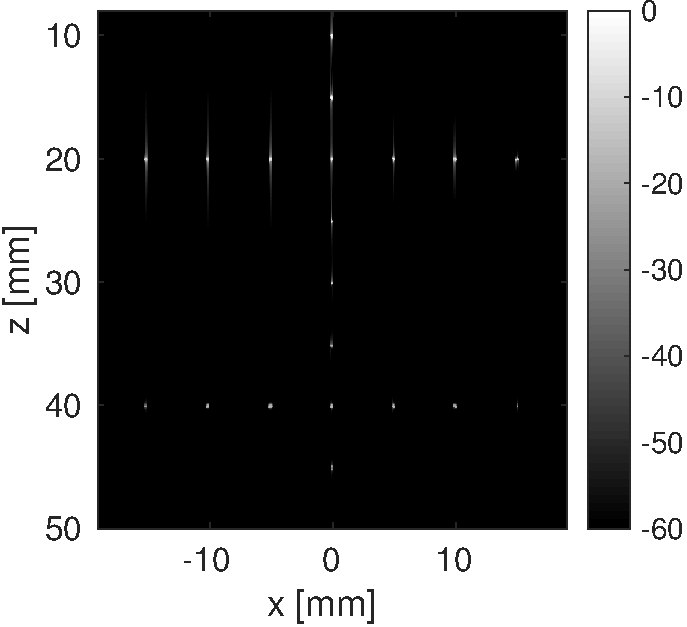
\includegraphics[height=\SimFigHeight]{figures/MCA_res_1PW.pdf}}\hfill%
	\caption{B-mode images for 1 PW insonification computed on the simulated contrast phantom reconstructed with (a) DAS and (b) the proposed approach, and on the simulated resolution phantom reconstructed with (c) DAS and (d) the proposed approach.}
	\label{fig:Bmode}
\end{figure*}
\subsection{Simulated contrast phantom}
\label{subsec_res_sim_contrast}
The number of segments has been set to $L = 6$. The thresholds for the shrinkage operators on each segments have been tuned manually. Since a threshold has to be fixed for each segment and each component, this amount to estimate $12$ thresholds. The value of $\epsilon$ has been set manually to respectively $0.89|| \bm{r} ||_2$, $0.89|| \bm{r} ||_2$ and $0.9|| \bm{r} ||_22$ for the three experiments. No transmit apodization has been used and a tapered cosine window ($F = 1.75$) has been used on receive. Since no bright reflector were present in the RF image, $\gamma$ has been set to 0.
The results, displayed in Figure 1(a), show a major increase of the contrast (around \SI{5}{\decibel}) compared to classical DAS for the three experiments. A visual assessment of the B-mode images on Figure \ref{fig:Bmode} confirms the higher quality of the reconstruction for the proposed approach.
\subsection{Experimental contrast phantom}
\label{subsec_res_exp_contrast}
The number of segments has been set to $L = 6$.  The value of $\epsilon$ has been set manually to respectively $0.92 || \bm{r} ||_2$, $0.85|| \bm{r} ||_2$ and $0.89|| \bm{r} ||_2$.  No transmit apodization has been used and a tapered cosine window ($F = 1.75$) has been used on receive. Eventually, since there was no bright reflector in the RF image, $\gamma$ has been set to 0.
The results, displayed in Figure 1(a), show a major increase of the contrast (around \SI{5}{\decibel}) compared to classical DAS for the three experiments.
\subsection{Simulated resolution phantom}
\label{subsec_res_sim_resolution}
The number of segments has been set to $L = 8$. The value of $\epsilon$ has been set manually to respectively $0.95 || \bm{r} ||_2$, $0.95 || \bm{r} ||_2$ and $0.96 || \bm{r} ||_2$.  No transmit apodization has been used on transmit and receive. Since there was no speckle in the RF image, $\gamma$ has been set to 1.
The results, displayed on Figures 1(b) and 1(c), show a major improvement of both the lateral and axial resolution compared to DAS for the three experiments. A visual assessment of the B-mode images on Figure \ref{fig:Bmode} confirms the better resolution obtained with the proposed approach.
\subsection{Experimental resolution phantom}
\label{subsec_res_exp_resolution}
The number of segments has been set to $L = 12$. The value of $\epsilon$ has been set manually to respectively $0.95 || \bm{r} ||_2$, $0.9 || \bm{r} ||_2$ and $0.95 || \bm{r} ||_2$.  No transmit apodization has been used on transmit and receive. Since there was no speckle in the RF image, $\gamma$ has been set to 1.
The results, displayed on Figures 1(b) and 1(c), show a major improvement of both the lateral and axial resolution compared to DAS for the three experiments. 
\subsection{Limits and perspective}
\label{subsec_limitation_prop_app}
The proposed approach outperforms existing classical DAS in terms of image quality. However, it suffers from several drawbacks. Firstly, the size of the matrix $\mathsf{H}$ may become prohibitive for compounding experiments. This is the main reason why the 75 PWs experiment have not been performed. Secondly, the number of parameters to evaluate is bigger than with classical sparse regularization. Indeed, a threshold value for the shrinkage operator has to be evaluated for each segment. The number of segments is also a parameter that has to be estimated. Empirically, segments of 10 to \SI{20}{\milli\metre} appear to be a good choice~\cite{BZhang_IUS_2015}.
In addition, the proposed approach is computationally heavy since the reconstruction algorithm is sub-iterative. Indeed, the projection on the $\ell_2-$ball of the constraint requires several iterations. For compounding experiments with a high number of SPWs, it makes the problem hardly tractable. A solution to such a problem would be to focus on primal dual algorithms~\cite{Komodakis_SPM_2015}.
%%%%%%%%%%%%%%%%%%%%%%%%%%%%%%%%%%%%%%%%%%%%%%%%%%%%%%%%%%%%%%%%%%%%%%%%%%%%%%%%
\section{Conclusion}
\label{sec:Conc}
In this study, a novel sparse regularization method is described which outperforms classical approaches in terms of contrast and resolution. A component-based model is introduced in which RF images are divided into bright reflector and background components, sparse in two different models. Spatial variability of the PSF is taken into account since US images are segmented in stripes in which the PSF is supposed to be quasi-stationary. The sparsity prior is then adapted to each stripe leading to unbiased optimization algorithm and higher image quality. 
\section*{Acknowledgements}
This work was supported in part by the UltrasoundToGo RTD project (no. 20NA21 145911), evaluated by the Swiss NSF and funded by Nano-Tera.ch with Swiss Confederation financing.
\bibliographystyle{ieeetr}
\bibliography{PICMUS_IUS2016}
\end{document}


